%% LaTeX2e class for student theses
%% sections/content.tex
%% 
%% Karlsruhe Institute of Technology
%% Institute for Program Structures and Data Organization
%% Chair for Software Design and Quality (SDQ)
%%
%% Dr.-Ing. Erik Burger
%% burger@kit.edu
%%
%% Version 1.3.3, 2018-04-17

\chapter{Background}
\label{ch:Background}

This chapter provides background information
on several concepts that are important to the rest of this thesis.
The sections below are not intended to be comprehensive introductions to the respective topics,
but focus on the aspects that are necessary to understand the thesis,
omitting parts that are unnecessary or distracting in this context.
Further information, including full introductions to most topics covered here,
can be found in the works listed in the bibliography.

\section{RDF}
\label{sec:Background:RDF}

\acrfull{rdf}
\cite{Lanthaler:14:RCA}
is a framework for describing and working with \gls{Linked Data},
developed by the \gls{rdf} Working Group under the umbrella of the \gls{w3c}.
In \gls{rdf}, information is arranged in \gls{subject}-\gls{predicate}-\gls{object} \glspl{triple},
such as “<Alan Turing> <is a> <human>”
or “<Lima> <was founded in> <18 January 1535>”.
All three elements of a \gls{triple} are typically \glspl{resource},
identified by an \gls{iri} like \url{http://example.com/Alan_Turing} or \url{http://www.wikidata.org/entity/Q5},
but the \gls{object} of a \gls{triple} can also be some other kind of value,
such as a textual, numerical or other literal
(e.~g. the date literal “18 January 1535” above).
A collection of such \glspl{triple} forms a directed, labeled graph,
where the \glspl{triple} describe individual edges
and the nodes are the \glspl{subject} and \glspl{object} of the \glspl{triple}:
\glspl{triple} with the same \gls{subject} constitute different outgoing arcs from the same node.
This graph can then be queried using the \acrfull{sparql} \cite{9569543}.
For a more detailed introduction to \gls{rdf} and related technologies,
see the RDF 1.1 Primer \cite{Schreiber:14:RP}.

To improve readability, the \glspl{iri} identifying a \gls{resource}
are usually abbreviated using \glspl{prefix}.
For example, once the \gls{prefix} \prefix{ex:} has been defined to mean \url{http://shex.example/},
the \glspl{iri} \url{http://shex.example/Person} and \url{http://shex.example/dateOfBirth}
can be abbreviated as \PName{ex:Person} and \PName{ex:dateOfBirth}.
(This “example” \gls{prefix}, also used below for other examples,
follows the naming conventions of schema.org \cite{schema.org-old-extension},
in that types (\PName{ex:Person}) and entities (\PName{ex:JohnDoe}) are in upper camel case
while predicates (\PName{ex:dateOfBirth}) are in lower camel case.)

While \gls{rdf} can be used with any \gls{resource} \glspl{iri},
one of its strengths is the ability to reuse the same \emph{vocabularies}
(effectively, sets of \glspl{resource})
in many different graphs.
For example, many graphs use the same \gls{predicate}, \PName{rdfs:label},
to link a \gls{resource} to a human-readable version of its name (its label);
a tool based on \gls{rdf} can thus offer human-readable names for \glspl{resource} from all these graphs
without requiring any specific knowledge about them,
and the graphs are more useful when used in combination.
One common vocabulary is \acrfull{rdfs} \cite{Guha:14:RS},
which among others provides two important predicates:
\PName{rdf:type} and \PName{rdfs:subClassOf}.
\PName{rdf:type} connects an object to its class,
and \PName{rdfs:subClassOf} connects a class to its parent class.
(The \prefix{rdf:} and \prefix{rdfs:} \glspl{prefix} are both part of \acrlong{rdfs};
the distinction between them is “a somewhat annoying historical artifact” \cite{Schreiber:14:RP}
with no real significance today.)
Another commonly used vocabulary is \gls{xsd} \cite{Malhotra:04:XSP},
which provides several basic datatypes:
for example, \PName{xsd:string} is the datatype for a simple text string (language-agnostic),
and \PName{xsd:date} and \PName{xsd:dateTime} are used to notate points in time.

\Cref{fig:rdf-example} shows a small example \gls{rdf} graph
for President Franklin D.~ Roosevelt and his pet dog, Fala.
The nodes with rounded corners represent \glspl{resource},
whereas the nodes with pointed corners are literals,
with their datatype given below them in parentheses.
Each arrow denotes a \gls{triple}, pointing from the \gls{subject} to the \gls{object},
with the \gls{predicate} written next to the arrow.
The graph describes the name and date of birth of the president and his dog,
their ownership relation,
and their types, including subtype relations:
Franklin D.~Roosevelt is a person, Fala is a dog,
and both persons and dogs are kinds of creatures.

The same graph may also be written textually in several syntaxes.
The simplest \gls{rdf} syntax is \gls{N-Triples} \cite{Seaborne:14:RN},
which lists \glspl{triple} one per line, each terminated with a period.
\Glspl{iri} are enclosed in angle brackets,
and literals are enclosed in double quotes,
optionally followed by two carets and their datatype
(otherwise the implied datatype is \PName{xsd:string}).
The \gls{N-Triples} representation of the same graph as in \cref{fig:rdf-example}
is presented in \cref{lst:rdf-example};
since \gls{N-Triples} does not allow the use of \glspl{prefix} to abbreviate \glspl{iri},
the \namecref{lst:rdf-example} has been rotated to fit the full width on the page.

\begin{figure}
  \centering
  \begin{tikzpicture}
    \tikzstyle{resource} = [rectangle, draw, rounded corners, text centered]
    \tikzstyle{literal} = [draw, text centered]
    \tikzstyle{arrow} = [draw, -latex']

    \begin{scope}
      \node[resource] (Creature) {\PName{ex:Creature}};
      \node[resource, below left=1cm and 1.5cm of Creature] (Human) {\PName{ex:Human}};
      \node[resource, below right=1cm and 1.5cm of Creature] (Dog) {\PName{ex:Dog}};
      \node[resource, below=1cm of Human] (FDR) {\PName{ex:FDR}};
      \node[resource, below=1cm of Dog] (Fala) {\PName{ex:Fala}};
    \end{scope}
    \begin{scope}[node distance=3cm, every text node part/.style={align=center}]
      \node[literal, below left of=FDR] (FDRDOB) {\graphRdfLiteral{1882-01-30}{xsd:date}};
      \node[literal, below of=FDR, node distance=4cm] (FDRName) {\graphRdfLiteral{Franklin Delano Roosevelt}{xsd:string}};
      \node[literal, below left of=Fala] (FalaName) {\graphRdfLiteral{Fala}{xsd:string}};
      \node[literal, below right of=Fala] (FalaDOB) {\graphRdfLiteral{1940-04-07}{xsd:date}};
    \end{scope}

    \begin{scope}[every path/.style=arrow, midway, auto]
      \path[left] (Human) -- node {\PName{rdfs:subClassOf}} (Creature);
      \path[right] (Dog) -- node {\PName{rdfs:subClassOf}} (Creature);
      \path[left] (FDR) -- node {\PName{rdf:type}} (Human);
      \path[right] (Fala) -- node {\PName{rdf:type}} (Dog);
      \path (FDR.north east) -- node {\PName{ex:pet}} (Fala.north west);
      \path (Fala.south west) -- node {\PName{ex:owner}} (FDR.south east);
      \path[left] (FDR) -- node {\PName{ex:dateOfBirth}} (FDRDOB);
      \path[right] (FDR) -- node {\PName{rdfs:label}} (FDRName);
      \path[left] (Fala) -- node {\PName{rdfs:label}} (FalaName);
      \path[right] (Fala) -- node {\PName{ex:dateOfBirth}} (FalaDOB);
    \end{scope}
  \end{tikzpicture}
  \caption{An \gls{rdf} graph for President Franklin D.~Roosevelt and his dog}
  \label{fig:rdf-example}
\end{figure}

\begin{sidewayslstfloat}
\begin{lstlisting}
<http://shex.example/FDR> <http://www.w3.org/1999/02/22-rdf-syntax-ns#type> <http://shex.example/Human>.
<http://shex.example/FDR> <http://www.w3.org/2000/01/rdf-schema#label> "Franklin Delano Roosevelt".
<http://shex.example/FDR> <http://shex.example/dateOfBirth> "1882-01-30"^^<http://www.w3.org/2001/XMLSchema#date>.
<http://shex.example/FDR> <http://shex.example/pet> <http://shex.example/Fala>.
<http://shex.example/Fala> <http://www.w3.org/1999/02/22-rdf-syntax-ns#type> <http://shex.example/Dog>.
<http://shex.example/Fala> <http://www.w3.org/2000/01/rdf-schema#label> "Fala".
<http://shex.example/Fala> <http://shex.example/dateOfBirth> "1940-04-07"^^<http://www.w3.org/2001/XMLSchema#date>.
<http://shex.example/Fala> <http://shex.example/owner> <http://shex.example/FDR>.
<http://shex.example/Human> <http://www.w3.org/2000/01/rdf-schema#subClassOf> <http://shex.example/Creature>.
<http://shex.example/Dog> <http://www.w3.org/2000/01/rdf-schema#subClassOf> <http://shex.example/Creature>.
\end{lstlisting}
\caption{An \gls{rdf} graph for President Franklin D.~Roosevelt and his dog}
\label{lst:rdf-example}
\end{sidewayslstfloat}

\section{Wikidata}
\label{sec:Background:Wikidata}

\Gls{Wikidata} \cite{Vrandecic:2014:WFC:2661061.2629489}
is a free knowledge base
and part of the \gls{Wikimedia} family of projects,
the most famous of which is \gls{Wikipedia}, the free encyclopedia.
Its contents are created, maintained and managed by the \gls{Wikidata} community,
most of whose members are volunteers,
as well as the members of other \gls{Wikimedia} projects, e.~g. \gls{Wikipedia}.
Anyone can contribute to \gls{Wikidata},
but the community ensures the quality of the contents with various quality control mechanisms.
Providing another such mechanism is part of the motivation for this thesis.

Information on \gls{Wikidata} is collected in \glspl{item},
which represent things or concepts:
there are \glspl{item} for individual persons,
for cities, states, geographical features,
for organizations and corporations,
\glspl{item} for books, films, newspapers, journals, scientific articles,
for abstract concepts, phenomena, emotions, philosophical movements, political orientations,
\glspl{item} for conceptual hierarchies, parent classes, biological taxa,
and even \glspl{item} for fictional characters, places, or other entities.

All of these \glspl{item} follow the same structure.
They are identified by their \gls{item ID},
a consecutive number prefixed with the letter “Q”
(e.~g. \Q{Q188709} for Beethoven’s Symphony No. 5).
They can have a \gls{label}, a \gls{description}, and \glspl{alias}, each in various languages:
for example, the \gls{item} \Q{Q7251} is labeled “Alan Turing” in English
but «\foreignlanguage{russian}{Алан Тьюринг}» in Russian;
is described as a “British mathematician, logician, cryptanalyst, and computer scientist” in English;
and may also be found under search aliases like “Alan M. Turing”, “Alan Mathison Turing” or simply “Turing”.
\Glspl{item} also have a set of \glspl{sitelink}
(links to pages about the same concept in various other \gls{Wikimedia} projects –
\gls{Wikipedia} articles, \gls{Wikiquote} pages, \gls{Wikimedia Commons} galleries, etc.),
and most importantly, a set of \glspl{statement}.

The \glspl{statement} are where most of the information in \gls{Wikidata} is stored.
They consist of a \gls{property}, such as “place of birth” or “author” or “population”,
and a value, which can be a reference to another \gls{item}, a quantity, a point in time, a piece of text,
or a few other possible types.
A \gls{statement} can also have \glspl{qualifier}
(further property-value pairs, e.~g. clarifying when or where the statement is valid)
and \glspl{reference} (sets of property-value pairs, listing sources for the \gls{statement}),
but those are mostly ignored in the context of this thesis.
\Glspl{property} are also identified by an ID, their \gls{property ID}
(prefixed with the letter “P” instead of “Q”),
and can also have \glspl{label}, \glspl{description} and \glspl{alias} in different languages:
for example, \P{P31} is labeled “instance of” in English
and „\foreignlanguage{ngerman}{ist ein(e)}“ in German.
The \glspl{label} and \glspl{description} are necessary to understand the meaning of \glspl{statement},
but they are not themselves part of the \glspl{statement}:
\glspl{statement} only list references to \gls{property} and \glspl{item ID},
making most of the information in \gls{Wikidata} language-agnostic \cite{Kaffee:2017:GBA:3125433.3125465}.

\Cref{fig:montblanc} shows two screenshots of the same \gls{Wikidata} \gls{item},
\QL{Q761735}{Montblanc}, viewed in different languages,
both as of \wikidataPermalink{704641959}.
The page structure is the same regardless of language:
first, there is a heading, showing the \gls{label} in the current language and the \gls{item ID};
below it on the left side is the “term box”,
listing \glspl{label}, \glspl{description} and \glspl{alias} in several languages relevant to the user;
below that is the list of \glspl{statement};
to the right are lists of \glspl{sitelink} for different \gls{Wikimedia} projects.
The screenshots are truncated
(the page has also been lightly edited for the screenshots
to remove some spacing and a few less relevant page elements)
and do not show the full list of \glspl{statement},
but the \glspl{statement} pictured are:
\begin{itemize}
\item A \gls{statement} for the \gls{property} \P{P31},
  where the value is an \gls{item}, \Q{Q33146843}.
\item A \gls{statement} for the \gls{property} \P{P18},
  where the value is a media file on \gls{Wikimedia Commons}.
  Image credit:
  \href{https://commons.wikimedia.org/wiki/User:Mariarosafg}{Mariarosafg}
  (\url{https://commons.wikimedia.org/wiki/File:Ciutat_de_Montblanc.jpg}),
  “Ciutat de Montblanc”,
  \url{https://creativecommons.org/licenses/by-sa/3.0/legalcode}
\item Two \glspl{statement} for the \gls{property} \P{P1448},
  where the values are monolingual text strings.
  Both \glspl{statement} also have \glspl{qualifier} and \glspl{reference}.
\end{itemize}
In \cref{fig:montblanc-en},
the \gls{item} is viewed as an anonymous user in the default English language
(German is shown as a second language in the term box
because the request was made from a German IP address;
logged in users can configure which languages they want to be shown here).
In \cref{fig:montblanc-ca},
the \gls{item} is viewed as an anonymous user, explicitly requested in the Catalan language:
notice that all \gls{property} and \gls{item} \glspl{label} are now different.

\begin{figure}
  \caption{Two screenshots of the same \gls{item} viewed in different languages}
  \label{fig:montblanc}
  \begin{subfigure}{\textwidth}
    \caption{The \gls{item} viewed as an anonymous user in the default English language}
    \label{fig:montblanc-en}
    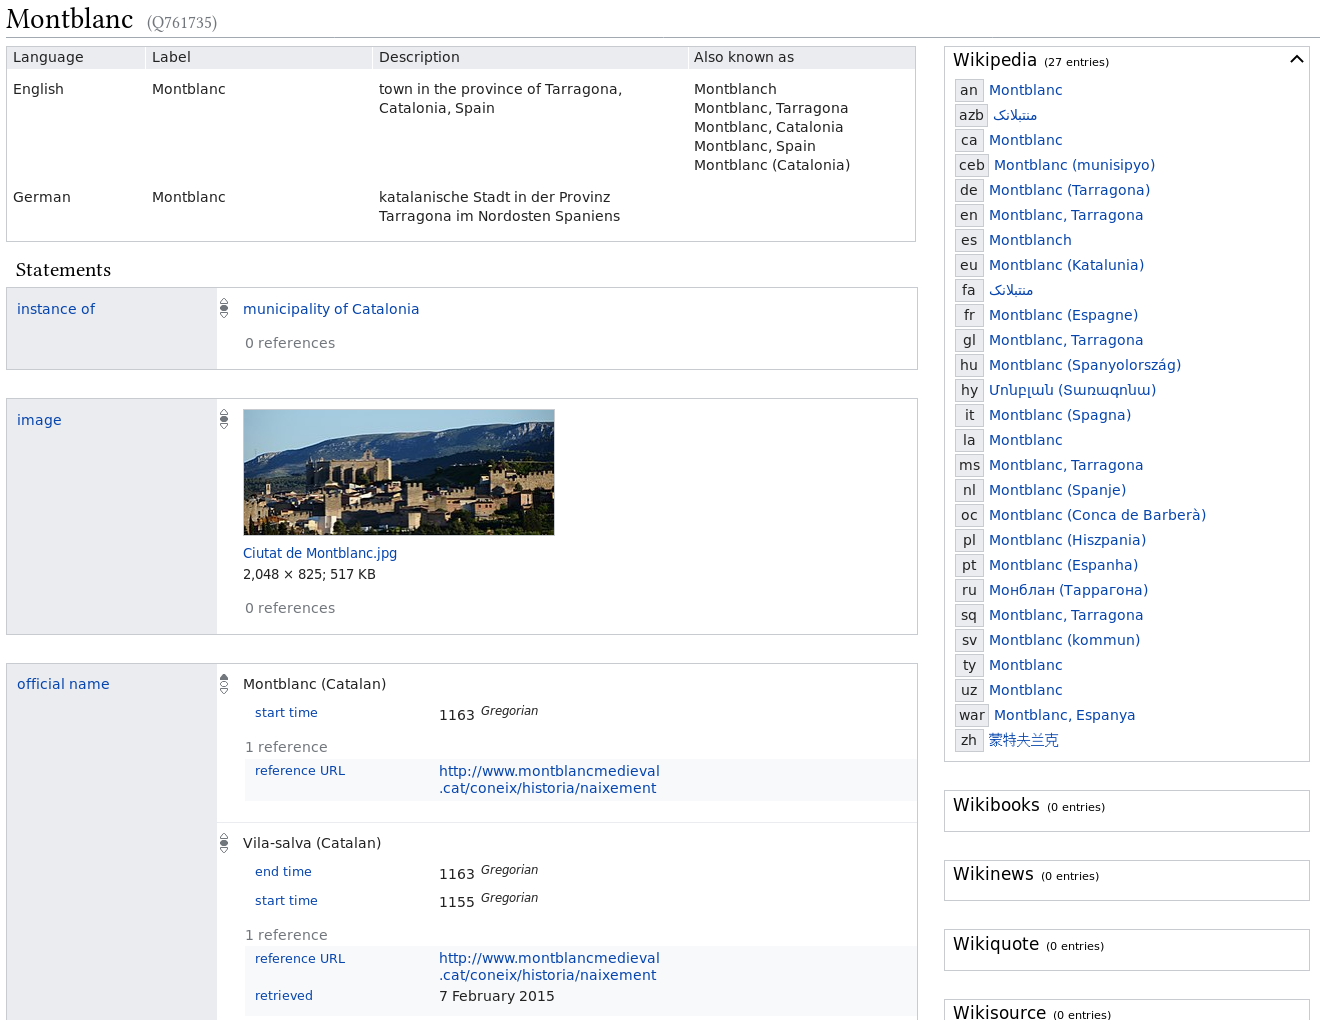
\includegraphics[width=\textwidth]{screenshots/montblanc-en}
  \end{subfigure}
\end{figure}
\begin{figure}\ContinuedFloat
  \begin{subfigure}{\textwidth}
    \caption{The \gls{item} viewed as an anonymous user, explicitly requested in the Catalan language}
    \label{fig:montblanc-ca}
    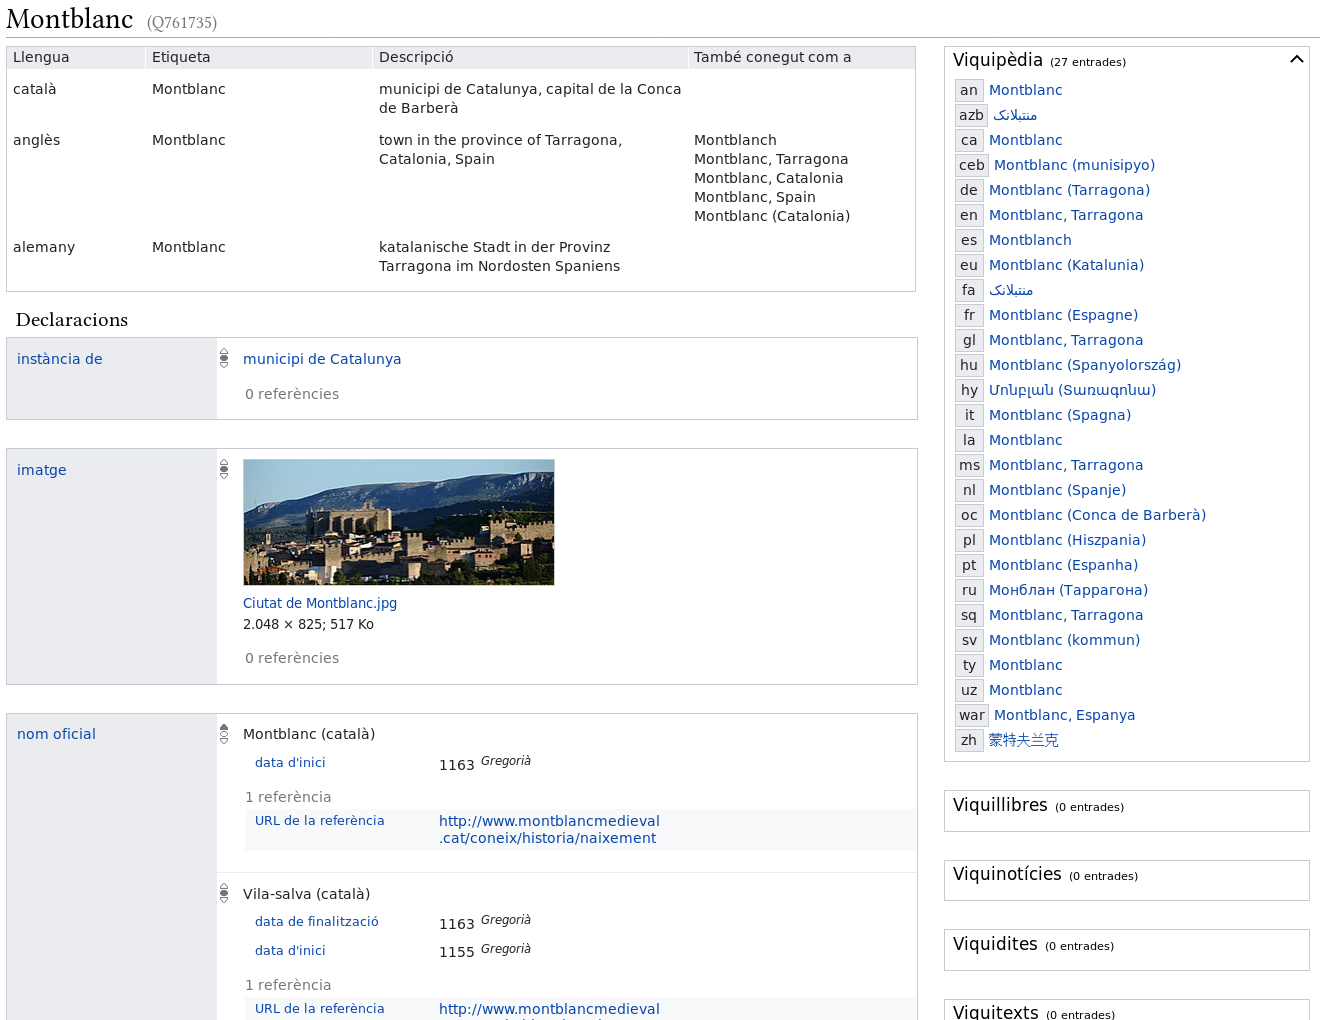
\includegraphics[width=\textwidth]{screenshots/montblanc-ca}
  \end{subfigure}
\end{figure}

It is vital to observe that there is no kind of \gls{schema} inherent to the \gls{Wikidata} data model.
Any \gls{property} can be used on any \gls{item}:
nothing in the software stops one from adding, say,
a “date of birth” \gls{statement} to an \gls{item} for a lake,
or a “parent taxon” \gls{statement} to an \gls{item} for a movie teaser poster.
The community has several ways to describe \glspl{schema} to varying degrees of formality
(such as \gls{property} lists on WikiProject pages or the property constraints system),
but they are all realized by community consensus,
not enforced by the \gls{Wikidata} software.
The great flexibility which this lends to the community
is considered to be one of \gls{Wikidata}’s greatest strengths \cite{vrandecic-restricting-the-world},
and though the use of \gls{shex}
on \gls{Wikidata} will provide another,
highly formal way to describe \glspl{schema},
there is no intention to change this fundamental operating principle of \gls{Wikidata}.

\Gls{Wikidata}’s data model, as described above,
is not directly related to \gls{rdf}.
However, to enable usage of \gls{rdf} technologies and interoperation with \gls{rdf}-based data sets,
\gls{Wikidata}’s data is exported to \gls{rdf}:
the data about any \gls{item} can be downloaded in various \gls{rdf} formats through a \gls{Linked Data} interface,
and a full, up-to-date \gls{rdf} export of \gls{Wikidata} is available in \gls{wdqs},
a \gls{sparql} endpoint to which anyone may submit queries.
In the \gls{Wikidata} \gls{rdf} exports,
items use the \gls{prefix} \prefix{wd:} and properties in a statement use the \gls{prefix} \prefix{wdt:}.
For example, the statement
\begin{quotation}
  \QL{Q7251}{Alan Turing}’s \PL{P19}{place of birth} was \QL{Q122744}{Maida Vale}
\end{quotation}
is represented in \gls{rdf} as the \gls{triple} \lstinline[language=sparql]{wd:Q7251 wdt:P19 wd:P12274}.
% TODO review layout of this statement/quote. (Using it inline is problematic because of ““double quotes””.)

% TODO explain some fundamental properties? P31, P279?

\section{Shape Expressions}
\label{sec:Background:ShEx}

% TODO somewhere, there needs to be a clear explanation why it’s so okay for us to constantly discard type links. here? not sure
% TODO example for validation

\acrfull{shex} \cite{shex}
is a standard for describing data shapes within an \gls{rdf} graph,
developed by the \gls{shex} Community Group under the umbrella of the \gls{w3c}.
A \gls{shex} \gls{schema} consists of a number of \glspl{shape},
each of which describes the layout of an \gls{rdf} \gls{resource},
called the \gls{focus node}.
The notation for \gls{shex} \glspl{schema} used in this thesis is \gls{shexc},
and while a full introduction to \gls{shex} and \gls{shexc} is beyond the scope of this thesis,
the relevant elements are described below.
For a more complete and detailed introduction,
see the \gls{shex} Primer \cite{shex-primer}.

In \gls{shexc}, a \gls{shape} definition begins with the \gls{shape}’s name (an \gls{iri})
and is followed by a block of \glspl{triple constraint} enclosed in curly braces (\lstinline!{}!).
The \glspl{triple constraint} are separated by semicolons (\lstinline{;})
and place restrictions on \glspl{triple} with the \gls{focus node} as the \gls{subject} and a certain \gls{predicate}:
a \gls{triple constraint} consists of the \gls{iri} for the \gls{predicate} and then a constraint on the \gls{object} (the value).
The value constraint can require the value to be a literal with a certain datatype,
expressed directly via the datatype’s \gls{iri},
or it can require the value to be a \gls{resource} matching another \gls{shape},
indicated by that \gls{shape}’s name (an \gls{iri}) following an \lstinline{@} symbol.
The value constraint may be followed by a cardinality for the \gls{triple constraint}:
instead of the default cardinality “must occur exactly once”,
the symbol \lstinline{?} may be appended to signify “zero or one times”
(an optional \gls{triple constraint}),
\lstinline{*} means “zero or more”
(any number of \glspl{triple} with this \gls{predicate} may occur,
but if they do occur, their \glspl{object} must still match the \gls{value constraint}),
and \lstinline{+} means “one or more”.
Multiple possible \glspl{triple constraint} for the same \gls{predicate} can be expressed
by grouping them inside parentheses (\lstinline{()}), separated by vertical bars (\lstinline{|}).

\begin{lstfloat}
\begin{lstlisting}[language=sparql]
ex:CreativeWork {
  ex:title rdf:langString;
  (
    ex:author @ex:Person+ |
    ex:author @ex:Organization
  );
  ex:cites @ex:CreativeWork*;
  ex:publicationDate xsd:dateTime?
}

ex:Person {
  ex:name rdf:langString;
  ex:dateOfBirth xsd:dateTime?
}

ex:Organization {
  ex:name rdf:langString+
}
\end{lstlisting}
\caption{An example \gls{schema} for creative works and their authors}
\label{listing:shex-example}
\end{lstfloat}

For example, the schema in \cref{listing:shex-example} defines three \glspl{shape}
for creative works and their authors.
It describes a creative work as having a title, a string in a certain language;
being written by one or more persons or an organization;
citing any number of other creative works;
and optionally having been published on a certain date and time.
(Scholarly articles would typically have human authors,
cite multiple works and have a publication date,
whereas a documentation page could be attributed to an organization as a whole
and have no significant citations or publication date.)
A person in this \gls{schema} has exactly one name in one language
(which is not generally true \cite{falsehoods-programmers-believe-about-names},
but violations of this should be rare enough
that they are worth investigating as potential errors)
and may have a date of birth, if known.
An organization does not have any properties other than at least one name
(it may have several, e.~g. in different languages or jurisdictions).

% TODO also add example of validation with results?

By default, \gls{shex} \glspl{shape} are not \emph{closed}:
the graph may contain additional \glspl{triple} with the \gls{focus node} as the \gls{subject}
whose \glspl{predicate} do not match any of the \glspl{triple constraint} in the \gls{shape}.
For example, an organization with an \PName{ex:dateOfIncorporation} would still match the \PName{ex:Organization} shape in \cref{listing:shex-example}
even though that \gls{schema} does not mention an \PName{ex:dateOfIncorporation} \gls{predicate} anywhere.
This means that removing all \glspl{triple constraint} with a certain \gls{predicate} from a \gls{shape}
will never cause a previously matching \gls{focus node} to no longer match the \gls{shape}.
% TODO I feel like this is missing one or two sentences at the end

\section{\gls{RDF2Graph}}
\label{sec:Background:RDF2Graph}

\Gls{RDF2Graph} \cite{vanDam2015}
is a tool to automatically determine the structure of an \gls{rdf} graph
and export it as a \gls{shex} \gls{schema}
(other output formats are also supported).
It relies heavily on the type information of each node and the class hierarchy in the graph,
determining the valid \glspl{predicate} and their value types and cardinalities for each type in the graph.
There is also an optional step to simplify the resulting \gls{schema}.

To discover the structure of an \gls{rdf} graph,
\gls{RDF2Graph} runs a set of queries against a \gls{sparql} endpoint serving that graph.
(This can be a local server, perhaps simply based on a single file containing the graph,
or a remote server.)
It enumerates all the classes that occur in the graph
and then collects all the \glspl{predicate} that are used on instances of each class.
For each \gls{predicate} of each class,
it then gets the types referenced in the values for those \glspl{predicate}
(usually the classes of the referenced nodes,
but values can also be literals or external references),
as well as forward and reverse multiplicity for each such type link.
All this information is stored in a separate \gls{rdf} graph private to \gls{RDF2Graph}.

If the simplification step is enabled,
\gls{RDF2Graph} will afterwards apply some transformations to the structure
based on the hierarchy of the classes involved,
which happens in several steps.
The following description uses the same step numbers as \cite{vanDam2015},
but elides several steps which are mostly implementation details,
which is why the step numbers are not consecutive here.
See \cite{vanDam2015} and the \gls{RDF2Graph} source code for the full description.
(In the source code, the steps are counted as sub-steps of the general step 7.4 “simplification”:
for example, step 2 is implemented under a code comment for “7.4.2”.)

% TODO review the layout of the listings here
% TODO some of the listings are too high for their page. perhaps remove blank lines between shapes

In step 2, all \glspl{predicate} from child classes are copied to parent classes.
For example, in \cref{fig:simplify-7.4.2},
the \PName{ex:WebResource} and \PName{ex:CreativeWork} classes are initially empty
but then inherit several \glspl{predicate} from their child classes.
(The \lstinline{.} in the \PName{ex:url} \gls{value constraint} means “any value”.)

\begin{lstfloat}[ht]
\begin{sublstfloat}[t]{0.45\textwidth}
\begin{lstlisting}[showlines=true]
ex:CreativeWork {}

ex:ScholarlyArticle
    EXTENDS ex:CreativeWork {
  ex:title rdf:langString;
  ex:author @ex:Person+;
  ex:cites @ex:CreativeWork+;
}

ex:WebResource
    EXTENDS ex:CreativeWork {}

ex:BlogPost
    EXTENDS ex:WebResource {
  ex:url .;
  ex:title rdf:langString;
  (
    ex:author @ex:Person |
    ex:author @ex:Organization
  );
}

ex:DocumentationPage
    EXTENDS ex:BlogPost {
  ex:url .;
  ex:title rdf:langString;
  ex:author @ex:Organization;
}















\end{lstlisting}
\caption{Before step 2}
\label{fig:simplify-7.4.2-before}
\end{sublstfloat}
\begin{sublstfloat}[t]{0.45\textwidth}
\begin{lstlisting}
ex:CreativeWork {
  ex:url .;
  ex:title rdf:langString;
  (
    ex:author @ex:Person+ |
    ex:author @ex:Organization
  );
  ex:cites @ex:CreativeWork+;
}

ex:ScholarlyArticle
    EXTENDS ex:CreativeWork {
  ex:title rdf:langString;
  ex:author @ex:Person+;
  ex:cites @ex:CreativeWork+;
}

ex:WebResource
    EXTENDS ex:CreativeWork {
  ex:url .;
  ex:title rdf:langString;
  (
    ex:author @ex:Person |
    ex:author @ex:Organization
  );
}

ex:BlogPost
    EXTENDS ex:WebResource {
  ex:url .;
  ex:title rdf:langString;
  (
    ex:author @ex:Person |
    ex:author @ex:Organization
  );
}

ex:DocumentationPage
    EXTENDS ex:WebResource {
  ex:url .;
  ex:title rdf:langString;
  ex:author @ex:Organization;
}
\end{lstlisting}
\caption{After step 2}
\label{fig:simplify-7.4.2-after}
\end{sublstfloat}
\caption[Simplification step 2]{Simplification step 2 (in \gls{shexc}-like pseudo-syntax)}
\label{fig:simplify-7.4.2}
\end{lstfloat}

Step 3 removes \glspl{predicate} which are only found in a single subclass
from the parent class again.
In the example from \cref{fig:simplify-7.4.2},
the \PName{ex:cites}  and \PName{ex:url} \glspl{predicate} will be removed from the \PName{ex:CreativeWork} \gls{shape}
because they are only found in one subclass
(\PName{ex:ScholarlyArticle} and \PName{ex:WebResource}, respectively),
while the other \glspl{predicate} will be kept.
In the \PName{ex:WebResource} \gls{shape} itself,
all \glspl{predicate} will be kept because they occur in both subclasses,
\PName{ex:BlogPost} and \PName{ex:DocumentationPage}.
See \cref{fig:simplify-7.4.3} for the result.

\begin{lstfloat}[ht]
\begin{sublstfloat}[t]{0.45\textwidth}
\begin{lstlisting}
ex:CreativeWork {
  ex:url .;
  ex:title rdf:langString;
  (
    ex:author @ex:Person+ |
    ex:author @ex:Organization
  );
  ex:cites @ex:CreativeWork+;
}

ex:ScholarlyArticle
    EXTENDS ex:CreativeWork {
  ex:title rdf:langString;
  ex:author @ex:Person+;
  ex:cites @ex:CreativeWork+;
}

ex:WebResource
    EXTENDS ex:CreativeWork {
  ex:url .;
  ex:title rdf:langString;
  (
    ex:author @ex:Person |
    ex:author @ex:Organization
  );
}

ex:BlogPost
    EXTENDS ex:WebResource {
  ex:url .;
  ex:title rdf:langString;
  (
    ex:author @ex:Person |
    ex:author @ex:Organization
  );
}

ex:DocumentationPage
    EXTENDS ex:WebResource {
  ex:url .;
  ex:title rdf:langString;
  ex:author @ex:Organization;
}
\end{lstlisting}
\caption{Before step 3}
\label{fig:simplify-7.4.3-before}
\end{sublstfloat}
\begin{sublstfloat}[t]{0.45\textwidth}
\begin{lstlisting}[showlines=true]
ex:CreativeWork {
  ex:title rdf:langString;
  (
    ex:author @ex:Person+ |
    ex:author @ex:Organization
  );
}

ex:ScholarlyArticle
    EXTENDS ex:CreativeWork {
  ex:title rdf:langString;
  ex:author @ex:Person+;
  ex:cites @ex:CreativeWork+;
}

ex:WebResource
    EXTENDS ex:CreativeWork {
  ex:url .;
  ex:title rdf:langString;
  (
    ex:author @ex:Person |
    ex:author @ex:Organization
  );
}

ex:BlogPost
    EXTENDS ex:WebResource {
  ex:url .;
  ex:title rdf:langString;
  (
    ex:author @ex:Person |
    ex:author @ex:Organization
  );
}

ex:DocumentationPage
    EXTENDS ex:WebResource {
  ex:url .;
  ex:title rdf:langString;
  ex:author @ex:Organization;
}


\end{lstlisting}
\caption{After step 3}
\label{fig:simplify-7.4.3-after}
\end{sublstfloat}
\caption[Simplification step 3]{Simplification step 3 (in \gls{shexc}-like pseudo-syntax)}
\label{fig:simplify-7.4.3}
\end{lstfloat}

After that, in step 4 all references which are still found in a parent class
are removed from the child classes, where they are now redundant.
In \cref{fig:simplify-7.4.4}, this mostly clears the \gls{schema}:
most \glspl{predicate} are found in \PName{ex:CreativeWork},
and only \PName{ex:WebResource} retains another \gls{predicate}, \PName{ex:url}.
Note that this step was later disabled, see \cref{sec:RDF2Graph+Wikidata:updates}.

\begin{lstfloat}[ht]
\begin{sublstfloat}[t]{0.45\textwidth}
\begin{lstlisting}
ex:CreativeWork {
  ex:title rdf:langString;
  (
    ex:author @ex:Person+ |
    ex:author @ex:Organization
  );
}

ex:ScholarlyArticle
    EXTENDS ex:CreativeWork {
  ex:title rdf:langString;
  ex:author @ex:Person+;
  ex:cites @ex:CreativeWork+;
}

ex:WebResource
    EXTENDS ex:CreativeWork {
  ex:url .;
  ex:title rdf:langString;
  (
    ex:author @ex:Person |
    ex:author @ex:Organization
  );
}

ex:BlogPost
    EXTENDS ex:WebResource {
  ex:url .;
  ex:title rdf:langString;
  (
    ex:author @ex:Person |
    ex:author @ex:Organization
  );
}

ex:DocumentationPage
    EXTENDS ex:WebResource {
  ex:url .;
  ex:title rdf:langString;
  ex:author @ex:Organization;
}
\end{lstlisting}
\caption{Before step 4}
\label{fig:simplify-7.4.4-before}
\end{sublstfloat}
\begin{sublstfloat}[t]{0.45\textwidth}
\begin{lstlisting}[showlines=true]
ex:CreativeWork {
  ex:title rdf:langString;
  (
    ex:author @ex:Person+ |
    ex:author @ex:Organization
  );
}

ex:ScholarlyArticle
    EXTENDS ex:CreativeWork {}

ex:WebResource
    EXTENDS ex:CreativeWork {
  ex:url .;
}

ex:BlogPost
    EXTENDS ex:WebResource {}

ex:DocumentationPage
    EXTENDS ex:WebResource {}




















\end{lstlisting}
\caption{After step 4}
\label{fig:simplify-7.4.4-after}
\end{sublstfloat}
\caption[Simplification step 4]{Simplification step 4 (in \gls{shexc}-like pseudo-syntax)}
\label{fig:simplify-7.4.4}
\end{lstfloat}

Step 2 also merges references to parent classes,
and the other steps take this into account by respecting subclass relations as well.
For example, consider the initial \gls{schema} in \cref{fig:simplify-classes}.
Initially, it states that scholarly articles only cite other scholarly articles,
and web resources only cite other web resources;
after simplification, it states that creative works cite other creative works of any kind:
the references to \PName{ex:ScholarlyArticle} and \PName{ex:WebResource}
were merged while copying the \PName{ex:cites} predicate into the \PName{ex:CreativeWork} parent class,
and afterwards the individual \glspl{predicate} were removed from the child classes
because they are covered by the merged reference in the parent class.

\begin{lstfloat}[ht]
\begin{sublstfloat}[t]{0.45\textwidth}
\begin{lstlisting}
ex:CreativeWork {}

ex:ScholarlyArticle
    EXTENDS ex:CreativeWork {
  ex:cites @ex:ScholarlyArticle+
}

ex:WebResource
    EXTENDS ex:CreativeWork {
  ex:cites @ex:WebResource*
}
\end{lstlisting}
\caption{Before simplification}
\label{fig:simplify-classes-before}
\end{sublstfloat}
\begin{sublstfloat}[t]{0.45\textwidth}
\begin{lstlisting}[showlines=true]
ex:CreativeWork {
  ex:cites @ex:CreativeWork*
}

ex:ScholarlyArticle
    EXTENDS ex:CreativeWork {}

ex:WebResource
    EXTENDS ex:CreativeWork {}


\end{lstlisting}
\caption{After simplification}
\label{fig:simplify-classes-after}
\end{sublstfloat}
\caption[Simplification, with class relations]{
  Simplification (in \gls{shexc}-like pseudo-syntax), with class relations
  (this example is independent from the previous example)
}
\label{fig:simplify-classes}
\end{lstfloat}

At this point, the information which \gls{RDF2Graph} extracted is available in a private \gls{rdf} graph.
From there, it can be exported into various formats by different exporters.
The \gls{shex} exporter loads parts of these results into a temporary \gls{rdf} database of its own,
applies some transformations to them via \gls{sparql},
converts them to \gls{json-ld},
further transforms the \gls{json},
and finally exports the result into \gls{shexc} text via the Jade template engine.

\section{Wikimedia Toolforge}
\label{sec:Background:Toolforge}

Wikimedia Toolforge is a hosting environment provided by the Wikimedia Foundation
where trusted members of the \gls{Wikimedia} community may host and develop their “tools” or other work.
Most tools are web-based and reachable under the \href{https://tools.wmflabs.org/}{tools.wmflabs.org} domain,
but it is also possible to run bots or analysis jobs on Toolforge.
Tools can be written in a variety of languages
(e.~g. PHP, Python, Java, \gls{JavaScript})
and have access to live replicas of the \gls{Wikimedia} production databases,
data dumps of \gls{Wikimedia} projects,
custom tool-specific databases,
and a Sun Grid Engine job execution system for long-running or resource-intensive tasks.
